% fig_tbanatomy.tex -- the four organs of a clocked testbench
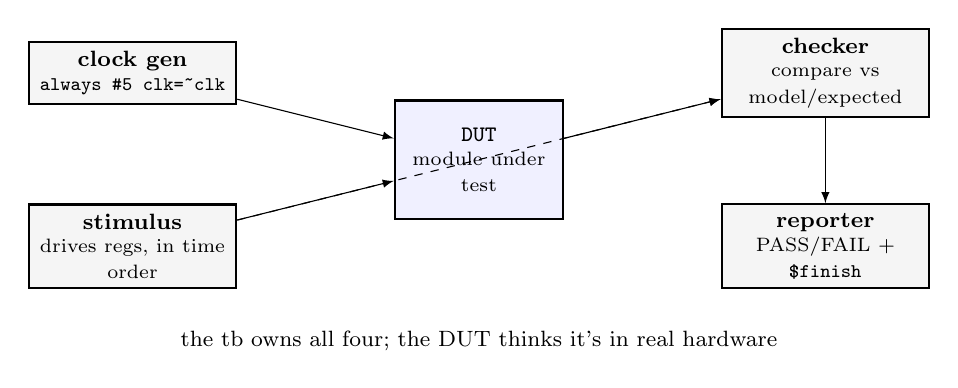
\begin{tikzpicture}[font=\footnotesize, >=latex]
  \node[draw, thick, fill=blue!6, minimum width=2.1cm, minimum height=1.5cm]
    (dut) at (0,0) {\parbox{1.9cm}{\centering \texttt{DUT}\\[-1pt]{\scriptsize module under test}}};
  \node[draw, thick, fill=gray!8, minimum width=2.6cm] (clk) at (-4.4,1.1)
    {\parbox{2.4cm}{\centering \textbf{clock gen}\\[-1pt]{\scriptsize\texttt{always \#5 clk=\textasciitilde clk}}}};
  \node[draw, thick, fill=gray!8, minimum width=2.6cm] (stim) at (-4.4,-1.1)
    {\parbox{2.4cm}{\centering \textbf{stimulus}\\[-1pt]{\scriptsize drives regs, in time order}}};
  \node[draw, thick, fill=gray!8, minimum width=2.6cm] (chk) at (4.4,1.1)
    {\parbox{2.4cm}{\centering \textbf{checker}\\[-1pt]{\scriptsize compare vs model/expected}}};
  \node[draw, thick, fill=gray!8, minimum width=2.6cm] (rpt) at (4.4,-1.1)
    {\parbox{2.4cm}{\centering \textbf{reporter}\\[-1pt]{\scriptsize PASS/FAIL + \texttt{\$finish}}}};
  \draw[->] (clk) -- (dut); \draw[->] (stim) -- (dut);
  \draw[->] (dut) -- (chk); \draw[->] (chk) -- (rpt);
  \draw[dashed, ->] (stim) -- (chk);
  \node[align=center] at (0,-2.3)
    {the tb owns all four; the DUT thinks it's in real hardware};
\end{tikzpicture}
